
\begin{enumerate}
    \item A cylindrical capillary tube of \(0.2 \, \text{mm}\) radius is made by joining two capillaries \(T1\) and \(T2\) of different materials having water contact angles of \(0^\circ\) and \(60^\circ\), respectively. The capillary tube is dipped vertically in water in two different configurations, case I and II as shown in figure. Which of the following option(s) is(are) correct?
        \begin{tasks}(2)
            \task The correction in the height of water column raised in the tube, due to weight of water contained in the meniscus, will be different for both cases.
            \task For case II, if the capillary joint is \(5 \, \text{cm}\) above the water surface, the height of water column raised in the tube will be \(3.75 \, \text{cm}\). (Neglect the weight of the water in the meniscus)
            \task For case I, if the joint is kept at \(8 \, \text{cm}\) above the water surface, the height of water column in the tube will be \(7.5 \, \text{cm}\). (Neglect the weight of the water in the meniscus)
            \task For case I, if the capillary joint is \(5 \, \text{cm}\) above the water surface, the height of water column raised in the tube will be more than \(8.75 \, \text{cm}\). (Neglect the weight of the water in the meniscus)
        \end{tasks}
\end{enumerate}
\begin{center}
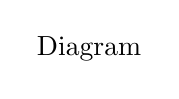
\begin{tikzpicture}
\node at (0,0) {Diagram};
\end{tikzpicture}
\end{center}
